% Training.tex: Training for hiragana and katakana
\ifthenelse{\equal{katakana}{\jtopic}}{%
\chapter{Katakana Training}\jchap{片仮名練習}\label{chap:KatakanaTraining}
\ithree{katakana!training}{片仮名練習}{Katakana!Training}
}{}
\ifthenelse{\equal{hiragana}{\jtopic}}{%
\chapter{Hiragana Training}\jchap{平仮名練習}\label{chap:HiraganaTraining}
\ithree{katakana!training}{平仮名練習}{Hiragana!Training}
}{}

\normalsize

Everyone learns in a different way. What works for one person may not work for
another. For this reason, an ultimate recipe for learning \textbf{\jtopic}
cannot be given here. However, the introduction to this chapter will try to
give some hints, gathered from learning and teaching experience.

\begin{description}

\item[Not too less:] If you learn one character per day, it will take about
        \jkanacount{} days for \textbf{\jtopic}. If you limit this to working
        days, it will take about two months. If you limit it to 2 hours per
        week, it will take a year to learn \textbf{\jtopic}. It is obvious
        that you are likely to forget the first characters while learning the
        last ones. But even with this method, it is not impossible, just
        unlikely.

\item[Not too much:] Learning \textbf{\jtopic} in one day is probably not
        possible. At least parts will be forgotten the next day.

\end{description}

In practice, the best results have been seen when students have tried to learn
\textbf{\jtopic} in one to three weeks. The suggestion is to learn one line
(five characters) per day in a cumulative way. That is, repeat the already
learned characters every day for up to 10 days until they are all learned. And
then repeat this exercise until they are almost impossible to forget. So for at
least 14 consecutive days without a break.

\begin{description}

\item[Develop your own style:] It is possible to learn one character at a time
        or one line (five characters at a time) or the whole table of
        \textbf{\jtopic}. It may take 3 weeks with one method or 1 week with
        another. It does not matter. What matters is that you feel comfortable
        with the method and that you have fun with it, even if you are forced
        to learn \textbf{\jtopic}. Decide for yourself how often to repeat. But
        decide. And write it down. Maybe even include it in your daily
        schedule. A good practice is to learn \textbf{\jtopic} 20 times a day
        for five minutes rather than once for three hours a day or once a week
        for 11 hours.

\item[Search for help:] Help can come in many forms. Of course, asking a
        Japanese person for help is useful. But there are many other ways to
        help yourself. One example is flash cards. Of course, it is easy to
        print them out in this book. But as I said before, find your own way.
        And if you make your own flashcards, you have already learned the
        content to a certain level.

\item[Use squares:] Some European languages use lines to teach letters. In
        Japanese, you should use a square and draw the letter in the middle. If
        you are unsure about the shape and orientation of the character, use a
        square and look at the squares filled with \textbf{\jtopic} in this
        section to understand the alignment and orientation.

\end{description}

\newpage

Here are some examples of flashcards. But feel free to design your own.

\begin{figure}[H]
        

\begin{center}
\begin{tabular}{cc}
\textbf{Front site rōmaji}&\textbf{Back site katakana}\\
\includegraphics[scale=1.5]{../share/i/fcar.pdf}% Rōmaji
&
\ifthenelse{\equal{hiragana}{\jtopic}}{
\includegraphics[scale=1.5]{../share/i/fcah.pdf}% Hiragana
}{}
\ifthenelse{\equal{katakana}{\jtopic}}{
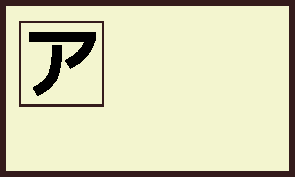
\includegraphics[scale=1.5]{../share/i/fcak.pdf}% Katakana
}{}
\\
\end{tabular}
\end{center}

        \caption{Flashcard type 1 (rōmaji - kana) }
        \label{fig:FlashCardTypeOne}
\end{figure}

\normalsize

Or to learn both:

\begin{figure}[H]
        \begin{center}
\begin{tabular}{cc}
\textbf{Front site rōmaji}&\textbf{Back site both}\\
\includegraphics[scale=1.5]{../share/i/fcar.pdf}% Rōmaji
&
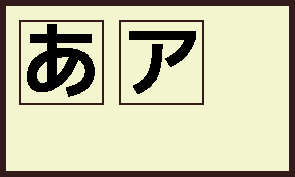
\includegraphics[scale=1.5]{../share/i/fcahk.pdf}% Hiragana/ Katakana
\\
\end{tabular}
\end{center}

        \caption{Flashcard type 2 (rōmaji - 2 kana)}
        \label{fig:FlashCardTypeTwo}
\end{figure}

\normalsize

Of course, skipping rōmaji is the preferred method to dive deep into Japanese:

\begin{figure}[H]
        \begin{center}
\begin{tabular}{cc}
\textbf{Front site Katakana}&\textbf{Back site Hiragana}\\
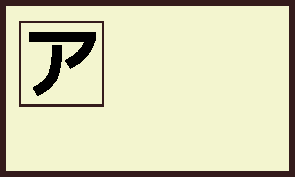
\includegraphics[scale=1.5]{../share/i/fcak.pdf}% Katakana
&
\includegraphics[scale=1.5]{../share/i/fcah.pdf}% Hiragana
\\
\end{tabular}
\end{center}

        \caption{Flashcard type 3 (katakana - hiragana)}
        \label{fig:FlashCardTypeThree}
\end{figure}

This training chapter can be used as an additional tool to learn
\textbf{\jtopic}. Again, it is important to develop your own method. However,
some hints for learning can be given with this training chapter.

\begin{description}

\item[Reading Loud:] When you write a \textbf{\jtopic} character in this book
        (and probably later), read the sound of the character out loud. Always.

\item[Invent your own cribs:] You can (maybe should?) invent one crib per
        character yourself. Especially if the character is hard to remember. It
        might be useful to write it down on the self-created flashcard for that
        specific character.

\item[Regular Repetition:] It is of course possible to fill in all fields for a
        character in a very short time. However, the learning effect should be
        minimal. It is better to fill in one row, then the second row an hour
        later, the third row the next day, and so on. The rhythm of repetition
        is up to you.

\item[Transcription:] Find a \textbf{\jtopic} text and read it. Write the Roman
        characters for each \jtopic{} word. If this is possible without looking
        up the \jtopic, then the transcription should be reversed. Find some
        Japanese text written in Rōmaji and transcribe it to \jtopic{} on 
        another piece of paper.

\end{description}

\newpage

                        % Katakana Hiragana
%----------------------------------------------------------------------------
\section{Katakana \jtl{a} Row}\jsec{片仮名ア行}\label{sec:KatakanaARow}

\Krow{arow}{a}{i}{u}{e}{o}

\label{letter:a}\KLETTER{a} The \jkatakana{} \jquotesingleja{ア} derives from
the \hyperref[sec:Radical]{radical} of the
\hyperref[sec:PhoneticCharacter]{phonetic character} \jquotesingleja{阿}.
Together with the \jkatakana{} \jquotesingleja{フ} \jtl{fu} the smaller sized
\jquotesingleja{ァ} gives the combination \jquotesingleja{ファ} and is
pronounced as such \jtl{fa}.

\label{letter:i}\KLETTER{i} The \jkatakana{} \jquotesingleja{イ} derives from
the \hyperref[sec:PhoneticCharacter]{phonetic characters} \jquotesingleja{伊}
left element (\hyperref[sec:Radical]{radical}). A smaller version
\jquotesingleja{ィ} is used in combinations with other letters and represents a
\hyperref[sec:Diphthong]{diphthong}.

\label{letter:u}\KLETTER{u} The \jkatakana{} \jquotesingleja{ウ} derives from
the \hyperref[sec:PhoneticCharacter]{phonetic character} \jquotesingleja{宇}. A
smaller version \jquotesingleja{ゥ} is used in combinations with other letters
and represents a \hyperref[sec:Diphthong]{diphthong} and is written as "w".
Even though the combination \jquotesingleja{トゥ} \jtl{tu} exist, it is
relatively new and many words do not use it. In this cases \jquotesingleja{ツ}
\jtl{tsu} is used. \jquotesingleja{ウ} can take \hyperref[sec:Dakuten]{dakuten}
to form \jquotesingleja{ヴ} \jtl{vu}, which is relatively new and can replace
\jquotesingleja{ブ} \jtl{bu}.

% UFuWaSimilarity
\subsection{\jtl{u}, \jtl{fu} and \jtl{wa} Similarity} \label{subsec:UFuWaSimilarity}

The Katakana characters \jquotesingleja{ウ}, \jquotesingleja{フ} and
\jquotesingleja{ワ} can be easily distinguished. All three have a different
stroke count. However the shape is similar. Therefore they can be mistaken.
Especially when they have no context.

\bigskip

\begin{figure}[H]
\begin{center}
\begin{tabular}{|c|c|c|}\hline
\KLETTER{u}&\KLETTER{fu}&\KLETTER{wa}\\\hline
\end{tabular}
\end{center}
\caption{\jtl{u}, \jtl{fu} and \jtl{wa} similarity}
\label{fig:UuFuAndWaSimilarity}
\end{figure}




\newpage

\label{letter:e}\KLETTER{e} The \jkatakana{} \jquotesingleja{エ} derives from
the \hyperref[sec:PhoneticCharacter]{phonetic characters} \jquotesingleja{江}
right element (\hyperref[sec:Radical]{radical}). A smaller version
\jquotesingleja{ェ} is used in combinations with other letters and express
\hyperref[sec:Mora]{morae} of foreign origin. For example \jquotesingleja{ヴェ}
is pronounced \jtl{ve}.

\label{letter:o}\KLETTER{o} The \jkatakana{} \jquotesingleja{オ} derives from
the \hyperref[sec:PhoneticCharacter]{phonetic character} \jquotesingleja{於}. A
smaller version \jquotesingleja{ォ} is used in combinations with other letters
and express' \hyperref[sec:Mora]{morae} of foreign origin. For example
\jquotesingleja{フォ } is pronounced \jtl{fo}.

\newpage

% ---------------------------------------------------------------------------
\subsection{\jtl{a}}\jsubsec{\jquotesingleja{ア}} \label{sec:KatakanaA}

\KatakanaHeader{a}{ The Katakana \jquotesingleja{ア} is written with two
        strokes. The first stroke starts horizontal. The second stroke is a
        curve with can be attached to the first stroke in hand writing, but not
        at the horizontal part - at the end of the first line.}
        \KatakanaTraining{a}

% ---------------------------------------------------------------------------
\subsection{\jtl{i}}\jsubsec{\jquotesingleja{イ}} \label{sec:KatakanaI}

\KatakanaHeader{i}{ The Katakana \jquotesingleja{イ} is written with one
stroke. The first stroke is a curve from upper right to lower left. The second
stroke is a vertical line attached to the first at the top.}
\KatakanaTraining{i}

% ---------------------------------------------------------------------------
\subsection{\jtl{u}}\jsubsec{\jquotesingleja{ウ}} \label{sec:KatakanaU}

\KatakanaHeader{u}{The Katakana \jquotesingleja{ウ} is written with three
strokes. The first stroke a small vertical line. The second a small vertical
line again and the third line a horizontal line connection the two others.}
\KatakanaTraining{u}

% ---------------------------------------------------------------------------
\subsection{\jtl{e}}\jsubsec{\jquotesingleja{エ}} \label{sec:KatakanaE}

\KatakanaHeader{e}{The Katakana \jquotesingleja{エ} is written with three
strokes. It is very geometrically consisting only out of horizontal and
vertical lines connected together.} \KatakanaTraining{e}

% ---------------------------------------------------------------------------
\subsection{\jtl{o}}\jsubsec{\jquotesingleja{オ}} \label{sec:KatakanaO}

\KatakanaHeader{o}{The Katakana \jquotesingleja{オ} is written with three
strokes. The first line is horizontal and together with the second stroke it
constructs a perfect crossing. The third stroke beginning lies at the center of
the crossing.} \KatakanaTraining{o}

% ---------------------------------------------------------------------------
\subsection{\jtl{a} Row Training}\jsubsec{片仮名ア行練習}
\Padding
\begin{longtable}[c]{p{2cm}p{2cm}p{3cm}p{6cm}p{2cm}}
\textit{Katakana}&\textit{Rōmaji}&\textit{Original}&\textit{Remark}&Origin\\\hline
ウエア&wuea&ware&          &English\\
エア  &ea  &air &          &English\\
エイ  &ei  &A   &the letter&English\\
\end{longtable}

\KanaSimpleTraining{Katakana to Rōmaji}{
\Transcribe{1.}{ウエア}{}{wear, ware}
\Transcribe{2.}{エア}{}{air}
\Transcribe{3.}{エイ}{}{A (the letter)}
\Transcribe{4.}{アイ}{}{I (the letter)}
\Transcribe{5.}{オウ}{}{O (the letter)}
%\Transcribe{6.}{イア}{}{ear}
}

\KanaSimpleTraining{Rōmaji to Katakana}{
\Transcribe{1.}{ea}{}{air}
\Transcribe{2.}{ai}{}{I (the letter)}
\Transcribe{3.}{ou}{}{O (the letter)}
\Transcribe{4.}{ei}{}{A (the letter)}
\Transcribe{5.}{uea}{}{wear, ware}
%\Transcribe{6.}{ia}{}{ear}
}

\newpage
\Padding
\begin{longtable}[c]{p{2cm}p{2cm}p{3cm}p{6cm}p{2cm}}
\textit{Katakana}&\textit{Rōmaji}&\textit{Original}&\textit{Remark}&Origin\\\hline
アイ  &ai  &I   &the letter&English\\
オウ  &ou  &O   &the letter&English\\
イア  &ia  &ear &          &English\\
\end{longtable}

\KanaSimpleTraining{English to Rōmaji}{
\Transcribe{1.}{ear}{}{}
\Transcribe{2.}{I (the letter)}{}{}
\Transcribe{3.}{air}{}{}
\Transcribe{4.}{O (the letter)}{}{}
\Transcribe{5.}{wear, ware}{}{}
%\Transcribe{6.}{A (the letter)}{}{}
}

\KanaSimpleTraining{English to Katakana}{
\Transcribe{1.}{I (the letter)}{}{}
\Transcribe{2.}{O (the letter)}{}{}
\Transcribe{3.}{air}{}{}
\Transcribe{4.}{ear}{}{}
\Transcribe{5.}{wear, ware}{}{}
%\Transcribe{6.}{A (the letter)}{}{}
}
\newpage
   % OK       OK
% ---------------------------------------------------------------------------
\section{Katakana \jtl{ka} Row}\jsec{片仮名カ行}\label{sec:KatakanaKaRow}

\Krow{karow}{ka}{ki}{ku}{ke}{ko}

\label{letter:ka}\KLETTER{ka} The  \textbf{katakana} \jquotesingleja{カ} is
pronounced \jtl{ka} and  derives from the
\hyperref[sec:PhoneticCharacter]{phonetic character}s \jquotesingleja{加} left
\hyperref[sec:Radical]{radical}.  A \hyperref[sec:Dakuten]{dakuten} version
exists and pronounced as \jtl{ga}.

%\hyperref[sec:Handakuten]{handakuten} does not exist in daily Japanese.
% \jquotesingleja{一ヵ所} {【いちかしょ】} (one place)
% \jquotesingleja{一ヶ所} {【いちかしょ】} (one place).
% 十ヵ条(十ヶ条)

\Note{Note}{

A smaller version \jquotesingleja{ヵ} is rare but used in combinations with
number particles.  For example in \jquotesingleja{一ヵ月} {【いっかげつ】} (one
month) and others.  This cases can also be written \jquotesingleja{一ヶ月}
{【いっかげつ】} (one month). Please see also \nameref{sec:KatakanaKe}. \Link
\href{https://ja.wikipedia.org/wiki/\%E3\%83\%B5}{ヵ}

}

\label{letter:ki}\KLETTER{ki} The \textbf{katakana} \jquotesingleja{キ} derives
from the \hyperref[sec:PhoneticCharacter]{phonetic character}s middle part of
either \jquotesingleja{機} or \jquotesingleja{幾}.  It is pronounced as
\jtl{ki}.  A \hyperref[sec:Dakuten]{dakuten} version exists and pronounced as
\jtl{gi}.


\label{letter:ku}\KLETTER{ku} The \textbf{katakana} \jquotesingleja{ク} derives
from the \hyperref[sec:PhoneticCharacter]{phonetic character}s left upper part
of \jquotesingleja{久}.  It is pronounced as \jtl{ku}.  A
\hyperref[sec:Dakuten]{dakuten} version exists and pronounced as \jtl{gu}.  A
smaller version exists, but is used for the Ainu Language.

\label{letter:ke}\KLETTER{ke} The \textbf{katakana} \jquotesingleja{ケ} derives
from the \hyperref[sec:PhoneticCharacter]{phonetic character}s upper and left
part of \jquotesingleja{介}.  It is pronounced as \jtl{ke}.  A
\hyperref[sec:Dakuten]{dakuten} version exists and pronounced as \jtl{ge}.  The
smaller version \jquotesingleja{ヶ} is explained in the following note.

\newpage

\Note{Note}{

A smaller version \jquotesingleja{ヶ} is rare but used in combinations with
number particles.  For example in \jquotesingleja{一ヶ月} {【いっかげつ】} (one
month) and others.  This cases can also be written \jquotesingleja{一ヵ月}
{【いっかげつ】} (one month). There are cases where only \jquotesingleja{ヶ}
can be written {七ヶ宿} {【シチカシュク】} (Place at the south west border of
the prefecture Miyagi).  In other rare cases this character can be pronounced
different \jquotesingleja{関ヶ原} {【せきがはら】} (Place at the south border
of the Gifu prefecture, known by the battle at 1600.). Please see also
\nameref{sec:KatakanaKa}. \Link
\href{https://ja.wikipedia.org/wiki/\%E3\%83\%B5}{ヵ}

}

\label{letter:ko}\KLETTER{ko} The \textbf{katakana} \jquotesingleja{コ} derives
from the \hyperref[sec:PhoneticCharacter]{phonetic character}s upper part of
\jquotesingleja{己}.  It is pronounced as \jtl{ko}.  A
\hyperref[sec:Dakuten]{dakuten} version exists and pronounced as \jtl{go}.



\newpage

% ---------------------------------------------------------------------------
\subsection{\jtl{ka}}\jsubsec{\jquotesingleja{カ}} \label{sec:KatakanaKa}

\KatakanaHeader{ka}{ \jtl{ka} is written with 2 strokes. Basically the same way
as the Hiragana \jquotesingleja{か} it looks like a squarish version, but
without the last stroke. The hook at the second stroke is less significant or
important.  } \KatakanaTraining{ka}

% ---------------------------------------------------------------------------
\subsection{\jtl{ki}}\jsubsec{\jquotesingleja{キ}} \label{sec:KatakanaKi}

\KatakanaHeader{ki}{ The shape alignment of the \jquotesingleja{キ} character
is not straight towards its environment. However the junctions are more or less
90 degrees.  } \KatakanaTraining{ki}

% ---------------------------------------------------------------------------
\subsection{\jtl{ku}}\jsubsec{\jquotesingleja{ク}} \label{sec:KatakanaKu}
% ---------------------------------------------------------------------------

\KatakanaHeader{ku}{ The first stroke is similar the stroke of
\jquotesingleja{ケ} is a curve. While the second stroke start aligned and
straight. } \KatakanaTraining{ku}

% ---------------------------------------------------------------------------
\subsection{\jtl{ke}}\jsubsec{\jquotesingleja{ケ}} \label{sec:KatakanaKe}

\KatakanaHeader{ke}{ The \jquotesingleja{ケ} is written with 3 strokes and the
first stroke is similar to the \jquotesingleja{ク}. The second stroke is
aligned and straight.  While the last stroke is a curve.  }
\KatakanaTraining{ke}

% ---------------------------------------------------------------------------
\subsection{\jtl{ko}}\jsubsec{\jquotesingleja{コ}} \label{sec:KatakanaKo}

\KatakanaHeader{ko}{ This character is almost a geometric figure composed out
of two strokes. However unless in European languages this are only 2 strokes
and not 3. The first stroke is the longest one and done similar with all
{漢字}. } \KatakanaTraining{ko}

% ---------------------------------------------------------------------------
\subsection{\jtl{ka} Row Training}\jsubsec{片仮名カ行練習}

\Padding
\begin{longtable}[c]{p{2cm}p{1.5cm}p{1.5cm}p{3cm}p{7cm}}
\textit{Katakana}&\textit{Rōmaji}&\textit{Original}&\textit{Remark}&Origin\\\hline
カキ  &kaki &kaki &柿 persimon&Japanese\\
ケア  &kea  &care &          &English\\
ケイ  &kei  &K    &the letter&English\\
\end{longtable}

\KanaSimpleTraining{Katakana to Rōmaji}{
\Transcribe{1.}{カキ}{}{persimmon}
\Transcribe{2.}{ココア}{}{cocoa}
\Transcribe{3.}{ケア}{}{care}
\Transcribe{4.}{コア}{}{core}
\Transcribe{5.}{ケーキ}{}{cake}
%\Transcribe{6.}{ケイ}{}{K (the letter)}
}

\KanaSimpleTraining{Rōmaji to Katakana}{
\Transcribe{1.}{kokoa}{}{cocoa}
\Transcribe{2.}{k$\overline{\mbox{e}}$ki}{}{cake}
\Transcribe{3.}{kea}{}{care}
\Transcribe{4.}{koa}{}{core}
\Transcribe{5.}{kaki}{}{persimmon}
%\Transcribe{6.}{kei}{}{K (the letter)}
}

\newpage

\Padding
%\begin{longtable}[c]{p{2cm}p{2cm}p{3cm}p{6cm}p{2cm}}
\begin{longtable}[c]{p{2cm}p{2.0cm}p{3.5cm}p{4cm}p{2.5cm}}
\textit{Katakana}&\textit{Rōmaji}&\textit{Original}&\textit{Remark}&Origin\\\hline
コア  &koa  &core &          &English\\
ココア&kokoa&cocoa& hot chocolate &English, from metathesis of Spanish cacao, from Nahuatl cacahuatl\\
ケーキ&kēki &cake &          &English\\
\end{longtable}


\KanaSimpleTraining{English to Rōmaji}{
\Transcribe{1.}{persimon}{}{}
\Transcribe{2.}{cocoa}{}{}
\Transcribe{3.}{care}{}{}
\Transcribe{4.}{core}{}{}
\Transcribe{5.}{K (the letter)}{}{}
%\Transcribe{6.}{cake}{}{}
}

\KanaSimpleTraining{English to Katakana}{
\Transcribe{1.}{cocoa}{}{}
\Transcribe{2.}{cake}{}{}
\Transcribe{3.}{care}{}{}
\Transcribe{4.}{persimon}{}{}
\Transcribe{5.}{K (the letter)}{}{}
%\Transcribe{6.}{core}{}{}
}

\newpage
  % OK
%----------------------------------------------------------------------------
\section{Katakana \jtl{sa} Row}\jsec{片仮名サ行}\label{sec:KatakanaSaRow}

\Krow{sarow}{sa}{shi}{su}{se}{so}

\label{letter:sa}\KLETTER{sa} The  \textbf{katakana} \jquotesingleja{サ} is
pronounced \jtl{sa} and derives from the
\hyperref[sec:PhoneticCharacter]{phonetic character}s \jquotesingleja{散} upper
left corner \hyperref[sec:Radical]{radical}.  A \hyperref[sec:Dakuten]{dakuten}
version exists and pronounced as \jtl{za}.

\label{letter:shi}\KLETTER{shi} The \textbf{katakana} \jquotesingleja{シ}
derives from the \hyperref[sec:PhoneticCharacter]{phonetic character} 
\jquotesingleja{之 }.  It is pronounced as \jtl{shi}.  A
\hyperref[sec:Dakuten]{dakuten} version exists and pronounced as \jtl{ji}.

\Note{Note}{Please see section \nameref{subsec:ShiTsuAmbiguity} for the
explanation how to write and distinguish \jtl{shi} and \jtl{tsu}.  }

\label{letter:su}\KLETTER{su} The \textbf{katakana} \jquotesingleja{ス} derives
from the \hyperref[sec:PhoneticCharacter]{phonetic character}s right lower part
of \jquotesingleja{須}.  It is pronounced as \jtl{su}.  A
\hyperref[sec:Dakuten]{dakuten} version exists and pronounced as \jtl{zu}.

\label{letter:se}\KLETTER{se} The \textbf{katakana} \jquotesingleja{セ} derives
from the \hyperref[sec:PhoneticCharacter]{phonetic character}s middle left part
of \jquotesingleja{世}.  It is pronounced as \jtl{se}.  A
\hyperref[sec:Dakuten]{dakuten} version exists and pronounced as \jtl{ze}.

\newpage

\label{letter:so}\KLETTER{so} The \textbf{katakana} \jquotesingleja{ソ} derives
from the \hyperref[sec:PhoneticCharacter]{phonetic character}s upper right part
of \jquotesingleja{曽}.  It is pronounced as \jtl{so}.  A
\hyperref[sec:Dakuten]{dakuten} version exists and pronounced as \jtl{zo}.

% SoRiNAmbiguity
\subsection{\jtl{so}, \jtl{ri} and \jtl{n} Ambiguity} \label{subsec:SoRiNAmbiguity}

The Katakana characters \jquotesingleja{ソ}, \jquotesingleja{リ} and
\jquotesingleja{ン} can be difficult to distinguish. All three are made out of
only 2 strokes. And especially \jtl{so} and \jtl{n} can be hard to tell. In a
sentence of course the context can help a lot.  But what are the rules for this
characters to write properly and distinguish?

\bigskip

\begin{figure}[H]
\begin{center}
\begin{tabular}{|c|c|c|}\hline
\KLETTER{so}&\KLETTER{n}&\KLETTER{ri}\\\hline
\end{tabular}
\end{center}
\caption{\jtl{so}, \jtl{ri} and \jtl{n} ambiguity}
\label{fig:SoRiAndNAmbiguity}
\end{figure}

\CharacterExplanation{soexplanation}{

To write the letter \jtl{so} it is important to align both lines
\textbf{horizontally} (red line) and to \textbf{non-align} the ends (blue line)
vertically. In this way it is possible to distinguish \jtl{so} from \jtl{n},
but not from \jtl{ri}. To also distinguish it from \jtl{ri} you have to write
the first stroke not horizontally nor vertically (green line).

}

\CharacterExplanation{nexplanation}{

To write the letter \jtl{n} it is important to a align both lines
\textbf{vertically} (red line) and to \textbf{non-align} the ends (blue line).
In this way it is possible to distinguish \jtl{n} from \jtl{so}. If both lines
are aligned there should not be a problem to distinguish it from \jtl{ri}.
Usually the angle of the green line is different, but only a small indicator.

}

\CharacterExplanation{riexplanation}{

To write the letter \jtl{ri} it is important to \textbf{align} both of the line
beginnings \textbf{horizontally} (red line) and to make sure that both lines
are \textbf{parallel} (green lines). There should be \textbf{no alignment} on
the left side (blue line) \textbf{vertically}. The difference between \jtl{so}
and \jtl{ri} is that \jtl{ri} need to start with two \textbf{parallel} lines
wile \jtl{so} should not. Please compare the left green line for an
explanation.

}



\newpage
% ---------------------------------------------------------------------------
\subsection{\jtl{sa}}\jsubsec{\jquotesingleja{サ}}\label{sec:KatakanaSa}

\KatakanaHeader{sa}{ Katakana \jquotesingleja{サ} is written with three
strokes. All crossings of strokes are in a 90 degree angle.  The starts of all
strokes are aligned either horizontally or vertically. The last stroke has a
curve.} \KatakanaTraining{sa}

% ---------------------------------------------------------------------------
\subsection{\jtl{shi}}\jsubsec{\jquotesingleja{シ}}\label{sec:KatakanaShi}

\KatakanaHeader{shi}{ The Katakana \jquotesingleja{シ} is written with three
strokes. All three strokes are aligned vertically in the beginning. Please see
section \nameref{subsec:ShiTsuAmbiguity}.} \KatakanaTraining{shi}

% ---------------------------------------------------------------------------
\subsection{\jtl{su}}\jsubsec{\jquotesingleja{ス}}\label{sec:KatakanaSu}

\KatakanaHeader{su}{The Katakana \jquotesingleja{ス} is written with two
strokes. The first stroke starts horizontally aligned. The second stroke
touches the first stroke at the beginning.} \KatakanaTraining{su}

% ---------------------------------------------------------------------------
\subsection{\jtl{se}}\jsubsec{\jquotesingleja{セ}}\label{sec:KatakanaSe}

\KatakanaHeader{se}{ The Katakana \jquotesingleja{セ} is written with two
strokes. The crossing has \textbf{no} 90 degree angle. The curve of the second
stroke as almost a 90 degree angle. } \KatakanaTraining{se}

% ---------------------------------------------------------------------------
\subsection{\jtl{so}}\jsubsec{\jquotesingleja{ソ}}\label{sec:KatakanaSo}

\KatakanaHeader{so}{ The Katakana \jquotesingleja{ソ} is written with two
strokes. The first stroke is not aligned vertically but it is aligned
horizontally withe the second stroke. Please see section
\nameref{subsec:SoRiNAmbiguity}.} \KatakanaTraining{so}

% ---------------------------------------------------------------------------
\subsection{\jtl{sa} Row Training}\jsubsec{片仮名サ行練習}\label{sec:SaRowTraining}
% 3 78 エキス
%3 357 スカイ
%3 360 スキー
%3 3 アイス
%3 111 ガーゼ
%3 146 イエス
\Padding
\begin{longtable}[c]{p{2cm}p{2cm}p{3cm}p{6cm}p{2cm}}
\textit{Katakana}&\textit{Rōmaji}&\textit{Original}&\textit{Remark}&\textit{Origin}\\\hline
エキス&ekisu&ex(tract)&extract&Dutch\\
スカイ&sukai&sky&&English\\
スキー&sukī&ski&noun for skiing&English\\
\end{longtable}
\KanaSimpleTraining{Katakana to Rōmaji}{
\Transcribe{1.}{エキス}{}{extract}      % ekisu
\Transcribe{2.}{スカイ}{}{sky}          % sukai
\Transcribe{3.}{スキー}{}{ski}          % sukī
\Transcribe{4.}{アイス}{}{ice}          % aisu
\Transcribe{5.}{ガーゼ}{}{gauze}        % gāze
%\Transcribe{6.}{イエス}{}{Jesus}        % iesu
}

\KanaSimpleTraining{Rōmaji to Katakana}{
\Transcribe{1.}{sukai}{}{sky}         % sukai
\Transcribe{2.}{ekisu}{}{extract}     % ekisu
\Transcribe{3.}{aisu}{}{ice}          % aisu
\Transcribe{4.}{suki}{}{ski}          % sukī
\Transcribe{5.}{iesu}{}{Jesus}        % iesu
%\Transcribe{6.}{gāze}{}{gauze}        % gāze
}

\newpage

\Padding
\begin{longtable}[c]{p{2cm}p{2cm}p{3cm}p{6cm}p{2cm}}
\textit{Katakana}&\textit{Rōmaji}&\textit{Original}&\textit{Remark}&Origin\\\hline
アイス&aisu&ice&water ice, ice cream&English\\
ガーゼ&gāze&Gaze&gauze&German\\
イエス&iesu&Jesus&Jesus&Portuguese\\
\end{longtable}
\KanaSimpleTraining{English to Rōmaji}{
\Transcribe{1.}{extract}{}{}       % ekisu
\Transcribe{2.}{sky}{}{}           % sukai
\Transcribe{3.}{Jesus}{}{}         % iesu
\Transcribe{4.}{gauze}{}{}         % gāze
\Transcribe{5.}{ice}{}{}           % aisu
%\Transcribe{6.}{ski}{}{}           % sukī
}

\KanaSimpleTraining{English to Katakana}{
\Transcribe{1.}{sky}{}{}           % sukai
\Transcribe{2.}{gauze}{}{}         % gāze
\Transcribe{3.}{ice}{}{}           % aisu
\Transcribe{4.}{Jesus}{}{}         % iesu
\Transcribe{5.}{extract}{}{}       % ekisu
%\Transcribe{6.}{ski}{}{}           % sukī
}

\newpage
  % OK
% ---------------------------------------------------------------------------
\section{Katakana \jtl{ta} Row}\jsec{片仮名タ行}\label{sec:KatakanaTaRow}

\Krow{tarow}{ta}{chi}{tsu}{te}{to}

\label{letter:ta}\KLETTER{ta} The  \textbf{katakana} \jquotesingleja{タ} is
pronounced \jtl{ta} and derives from the
\hyperref[sec:PhoneticCharacter]{phonetic character}s \jquotesingleja{多 }
upper or lover \hyperref[sec:Radical]{radical}.  A
\hyperref[sec:Dakuten]{dakuten} version exists and pronounced as \jtl{da}.

\label{letter:chi}\KLETTER{chi} The \textbf{katakana} \jquotesingleja{チ}
derives from the \hyperref[sec:PhoneticCharacter]{phonetic character} 
\jquotesingleja{千}.  It is pronounced as \jtl{chi}.  A
\hyperref[sec:Dakuten]{dakuten} version exists and pronounced as \jtl{ji}.

\label{letter:tsu}\KLETTER{tsu} The \textbf{katakana} \jquotesingleja{ツ}
derives from the \hyperref[sec:PhoneticCharacter]{phonetic character}s
\jquotesingleja{州} or \jquotesingleja{川} .  It is pronounced as \jtl{tsu}.  A
\hyperref[sec:Dakuten]{dakuten} version exists and pronounced as \jtl{zu}.

\label{letter:te}\KLETTER{te} The \textbf{katakana} \jquotesingleja{テ} derives
from the \hyperref[sec:PhoneticCharacter]{phonetic character}s lower left part
of \jquotesingleja{天 }.  It is pronounced as \jtl{te}.  A
\hyperref[sec:Dakuten]{dakuten} version exists and pronounced as \jtl{de}.

\newpage

\label{letter:to}\KLETTER{to} The \textbf{katakana} \jquotesingleja{ト} derives
from the \hyperref[sec:PhoneticCharacter]{phonetic character}s right part of
\jquotesingleja{止}.  It is pronounced as \jtl{to}.  A
\hyperref[sec:Dakuten]{dakuten} version exists and pronounced as \jtl{do}.

% ShiTsuAmbiguity
\subsection{\jtl{shi} and \jtl{tsu} Ambiguity} \label{subsec:ShiTsuAmbiguity}

% シ
% ツ

The Katakana characters \jquotesingleja{シ} and \jquotesingleja{ツ} are
difficult to distinguish.  Both are made out of 3 strokes and even the length
are equal. In a sentence of course the context can help a lot. But what are the
rules for this characters to write properly and distinguish?

\bigskip

\begin{figure}[H]
\begin{center}
\begin{tabular}{|c|c|}\hline
\KLETTER{shi}&\KLETTER{tsu}\\\hline
\end{tabular}
\end{center}
\caption{\jtl{shi} and \jtl{tsu} ambiguity}
\label{fig:ShiAndTsuAmbiguity}
\end{figure}

\CharacterExplanation{shiexplanation}{

To write the letter \jtl{shi} it is important to align three lines
\textbf{vertically} (red line) and to \textbf{non-align} the ends (blue line).
In this way it is possible to distinguish \jtl{shi} from \jtl{tsu}. Of course
also the angle of the frist two lines are different, but in hadwriting this is
difficult to match. As a rule of thumb make the third line double as long as
the first two but short enough to not align it at the end.

}

\CharacterExplanation{tsuexplanation}{

To write the letter \jtl{tsu} it is important to align all tree lines
\textbf{horizontally} (red line) and to \textbf{non-align} the ends (blue
line). In this way it is possible to distinguish \jtl{tsu} from \jtl{shi}. Of
course also the angle of the first two lines are different, but in handwriting
this is difficult to match. As a rule of thumb make the third line double as
long as the first two but short enough to not align it at the end.

}



\newpage

% ---------------------------------------------------------------------------
\subsection{\jtl{ta}}\jsubsec{\jquotesingleja{タ}}\label{sec:KatakanaTa}

\KatakanaHeader{ta}{ Katakana \jtl{ta} is written with three strokes. The first
stroke is a small curve. The secosnd stroke starts horizontally attached to the
first stroke. The third stroke ends at the second stroke.}
\KatakanaTraining{ta}

% ---------------------------------------------------------------------------
\subsection{\jtl{chi}}\jsubsec{\jquotesingleja{チ}}\label{sec:KatakanaChi}

\KatakanaHeader{chi}{ Katakana \jtl{chi} is written with three strokes. The
first stroke is a light curve. The second ihorizontally straight line. The
third line is a curve that joints the first and the second.}
\KatakanaTraining{chi}

% ---------------------------------------------------------------------------
\subsection{\jtl{tsu}}\jsubsec{\jquotesingleja{ツ}}\label{sec:KatakanaTsu}

\KatakanaHeader{tsu}{Katakana \jtl{tsu} is written with three strokes. The
first and second stroke are short. And the beginning of all three strokes is
aligned horizontally. The third stroke is the longest, but the end is not
alignd wit the beginning of the first stroke. } \KatakanaTraining{tsu}

% ---------------------------------------------------------------------------
\subsection{\jtl{te}}\jsubsec{\jquotesingleja{テ}}\label{sec:KatakanaTe}

\KatakanaHeader{te}{ Katakana \jtl{te} is written with three strokes. The first
stroke is the shortest and horizontally. The second stroke is not aligned
vertically in the beginning, but also perfectly horizontally. The third stroke
is a small curve attached to the middle of the second stroke. }
\KatakanaTraining{te}

% ---------------------------------------------------------------------------
\subsection{\jtl{to}}\jsubsec{\jquotesingleja{ト}}\label{sec:KatakanaTo}

\KatakanaHeader{to}{ Katakana \jtl{to} is written with 2 strokes. The first
stroke is a vertical line. Attached to this line there is short straight line
to the right. In some hand writings this line is a small curve to the right.}
\KatakanaTraining{to}

% ---------------------------------------------------------------------------
\subsection{\jtl{ta} Row Training}\jsubsec{片仮名タ行練習}
\Padding
\begin{longtable}[c]{p{2cm}p{2cm}p{3cm}p{6cm}p{2cm}}
\textit{Katakana}&\textit{Rōmaji}&\textit{Original}&\textit{Remark}&\textit{Origin}\\\hline
エステ        &esutei    &esthé(tique)&beauty salon, esthetic clinic    &French\\
サイト        &saito     &site        &&English\\
タスク        &tasuku    &task        &&English\\
\end{longtable}

\KanaSimpleTraining{Katakana to Rōmaji}{
\Transcribe{1.}{エステ}{}{esthé(tique)}
\Transcribe{2.}{サイト}{}{site}
\Transcribe{3.}{タスク}{}{task}
\Transcribe{4.}{テスト}{}{test}
\Transcribe{5.}{スーツアクター}{}{suit actor}
%\Transcribe{6.}{テキスト}{}{text}
}

\KanaSimpleTraining{Rōmaji to Katakana}{
\Transcribe{1.}{saito}{}{site}
\Transcribe{2.}{tasuku}{}{task}
\Transcribe{3.}{esute}{}{esthé(tique)}
\Transcribe{4.}{sūtsuakutā}{}{suit actor}
\Transcribe{5.}{tesuto}{}{test}
%\Transcribe{6.}{テキスト}{}{text}
}

\newpage
\Padding
\begin{longtable}[c]{p{2.6cm}p{2cm}p{1.8cm}p{6.6cm}p{1.8cm}}
\textit{Katakana}&\textit{Rōmaji}&\textit{Original}&\textit{Remark}&\textit{Origin}\\\hline
テスト        &tesuto    &test        &                                 &English\\
スーツアクター&sūtsuakutā&suit actor  &wearing cartoon-character costume&English\\
テキスト      &tekisuto  &text        &                                 &English\\
\end{longtable}

\KanaSimpleTraining{English to Rōmaji}{
\Transcribe{1.}{task}{}{}
\Transcribe{2.}{esthé(tique)}{}{}
\Transcribe{3.}{text}{}{}
\Transcribe{4.}{test}{}{}
\Transcribe{5.}{suit actor}{}{}
%\Transcribe{6.}{site}{}{}
}

\KanaSimpleTraining{English to Katakana}{
\Transcribe{2.}{esthé(tique)}{}{}
\Transcribe{4.}{test}{}{}
\Transcribe{5.}{suit actor}{}{}
\Transcribe{3.}{text}{}{}
\Transcribe{6.}{site}{}{}
%\Transcribe{1.}{task}{}{}
}

\newpage
  % OK
% ---------------------------------------------------------------------------
\section{Katakana \jtl{na} Row}\jsec{片仮名ナ行}\label{sec:KatakanaNaRow}

\Krow{narow}{na}{ni}{nu}{ne}{no}

\label{letter:na}\KLETTER{na} The  \textbf{katakana} \jquotesingleja{ナ} is
pronounced \jtl{na} and  derives from the
\hyperref[sec:PhoneticCharacter]{phonetic character}s \jquotesingleja{奈} upper
left corner part.  A \hyperref[sec:Dakuten]{dakuten} version  or
\hyperref[sec:Handakuten]{handakuten} do not exist.

\label{letter:ni}\KLETTER{ni} The  \textbf{katakana} \jquotesingleja{ニ} is
pronounced \jtl{ni} and  derives from the
\hyperref[sec:PhoneticCharacter]{phonetic character}s \jquotesingleja{奈} upper
right part.  A \hyperref[sec:Dakuten]{dakuten} version  or
\hyperref[sec:Handakuten]{handakuten} do not exist.

\label{letter:nu}\KLETTER{nu} The  \textbf{katakana} \jquotesingleja{ヌ} is
pronounced \jtl{nu} and  derives from the
\hyperref[sec:PhoneticCharacter]{phonetic character}s \jquotesingleja{奴} right
part.  A \hyperref[sec:Dakuten]{dakuten} version  or
\hyperref[sec:Handakuten]{handakuten} do not exist.

\Note{Note}{%

The characters \hyperref[letter:no]{\jquotesingleja{ノ}},
\hyperref[letter:me]{\jquotesingleja{メ}} and
\hyperref[letter:nu]{\jquotesingleja{ヌ}} are similar and it is easy to make a
mistake. To distinguish \jquotesingleja{メ} it is important to make all strokes
long enough.

}%


\newpage

\label{letter:ne}\KLETTER{ne} The  \textbf{katakana} \jquotesingleja{ネ} is
pronounced \jtl{ne} and  derives from the
\hyperref[sec:PhoneticCharacter]{phonetic character}s \jquotesingleja{祢} upper
left  part.  A \hyperref[sec:Dakuten]{dakuten} version  or
\hyperref[sec:Handakuten]{handakuten} do not exist.

\label{letter:no}\KLETTER{no} The  \textbf{katakana} \jquotesingleja{ノ} is
pronounced \jtl{no} and  derives from the
\hyperref[sec:PhoneticCharacter]{phonetic character}s \jquotesingleja{乃} upper
left part.  A \hyperref[sec:Dakuten]{dakuten} version  or
\hyperref[sec:Handakuten]{handakuten} do not exist.

\Note{Note}{%

The characters \hyperref[letter:no]{\jquotesingleja{ノ}},
\hyperref[letter:me]{\jquotesingleja{メ}} and
\hyperref[letter:nu]{\jquotesingleja{ヌ}} are similar and it is easy to make a
mistake. To distinguish \jquotesingleja{メ} it is important to make all strokes
long enough.

}%

\newpage

% ---------------------------------------------------------------------------
\subsection{\jtl{na}}\jsubsec{\jquotesingleja{ナ}} \label{sec:KatakanaNa}

\KatakanaHeader{na}{ Katakana \jtl{na} is written with two strokes.} \KatakanaTraining{na}

% ---------------------------------------------------------------------------
\subsection{\jtl{ni}}\jsubsec{\jquotesingleja{ニ}} \label{sec:KatakanaNi}

\KatakanaHeader{ni}{ Katakana \jtl{ni} is written with two strokes.} \KatakanaTraining{ni}

% ---------------------------------------------------------------------------
\subsection{\jtl{nu}}\jsubsec{\jquotesingleja{ヌ}} \label{sec:KatakanaNu}

\KatakanaHeader{nu}{Katakana \jtl{nu} is written with two strokes.} \KatakanaTraining{nu}

% ---------------------------------------------------------------------------
\subsection{\jtl{ne}}\jsubsec{\jquotesingleja{ネ}} \label{sec:KatakanaNe}

\KatakanaHeader{ne}{Katakana \jtl{ne} is written with three strokes.} \KatakanaTraining{ne}

% ---------------------------------------------------------------------------
\subsection{\jtl{no}}\jsubsec{\jquotesingleja{ノ}} \label{sec:KatakanaNo}

\KatakanaHeader{no}{Katakana \jtl{no} is written with one stroke.} \KatakanaTraining{no}

% ---------------------------------------------------------------------------
\subsection{ \jtl{na} Row Training}\jsubsec{片仮名ナ行練習}
\Padding
\begin{longtable}[c]{p{2cm}p{2cm}p{3cm}p{6cm}p{2cm}}
\textit{Katakana}&\textit{Rōmaji}&\textit{Original}&\textit{Remark}&\textit{Origin}\\\hline
ナース  &nāsu &nurse      &                                        &English\\
ネット  &netto&net(work)  &                                        &English\\
アニス &anisu&anise      &pimpinella anisum                       &\\
\end{longtable}

\KanaSimpleTraining{Katakana to Rōmaji}{
\Transcribe{1.}{ネット}{}{net(work)}
\Transcribe{2.}{ナース}{}{nurse}
\Transcribe{3.}{アニス}{}{anise}
\Transcribe{4.}{ニート}{}{NEET}
\Transcribe{5.}{ナイター}{}{night + -er}
%\Transcribe{6.}{ノート}{}{note}
}

\KanaSimpleTraining{Rōmaji to Katakana}{
\Transcribe{1.}{nōto}{}{note}
\Transcribe{2.}{netto}{}{net(work)}
\Transcribe{3.}{anisu}{}{anise}
\Transcribe{4.}{nāsu}{}{nurse}
\Transcribe{5.}{naitā}{}{night + -er}
%\Transcribe{4.}{ニート}{}{NEET}
}

\newpage
\Padding
\begin{longtable}[c]{p{2cm}p{2cm}p{3cm}p{6cm}p{2cm}}
\textit{Katakana}&\textit{Rōmaji}&\textit{Original}&\textit{Remark}&\textit{Origin}\\\hline
ニート  &nīto &NEET       &Not in Education, Employment or Training&English\\
ナイター&naitā&night + -er&     a night game                       &English\\
ノート  &nōto &note       & note, notebook                         &English\\
\end{longtable}
\KanaSimpleTraining{English to Rōmaji}{
\Transcribe{1.}{anise}{}{}
\Transcribe{2.}{net(work)}{}{}
\Transcribe{3.}{note}{}{}
\Transcribe{4.}{nurse}{}{}
\Transcribe{5.}{NEET}{}{}
%\Transcribe{5.}{night + -er}{}{}
}

\KanaSimpleTraining{English to Katakana}{
\Transcribe{1.}{nurse}{}{}
\Transcribe{2.}{note}{}{}
\Transcribe{3.}{net(work)}{}{}
\Transcribe{4.}{anise}{}{}
\Transcribe{5.}{night + -er}{}{}
%\Transcribe{4.}{NEET}{}{}
}

\newpage
  %
% ---------------------------------------------------------------------------
\section{ Katakana \jtl{ha} Row}\jsec{片仮名ハ行}\label{sec:KatakanaHaRow}

\Krow{harow}{ha}{hi}{fu}{he}{ho}

\label{letter:ha}\KLETTER{ha} The \textbf{katakana} \jquotesingleja{ハ} is
pronounced \jtl{ha} and derives from the
\hyperref[sec:PhoneticCharacter]{phonetic character} \jquotesingleja{八 }.  A
\hyperref[sec:Dakuten]{dakuten} version exists and pronounced as \jtl{ba}.

\label{letter:hi}\KLETTER{hi} The \textbf{katakana} \jquotesingleja{ヒ} derives
from the \hyperref[sec:PhoneticCharacter]{phonetic characters}
\jquotesingleja{比} reight \hyperref{sec:Radical}{radical}. It is pronounced as
\jtl{hi}. A \hyperref[sec:Dakuten]{dakuten} version exists and pronounced as
\jtl{bi}.

\label{letter:fu}\KLETTER{fu} The \textbf{katakana} \jquotesingleja{フ} derives
from the \hyperref[sec:PhoneticCharacter]{phonetic characters} upper left part
of \jquotesingleja{不 }. It is pronounced as \jtl{fu}. A
\hyperref[sec:Dakuten]{dakuten} version exists and pronounced as \jtl{bu}.

\label{letter:he}\KLETTER{he} The \textbf{katakana} \jquotesingleja{ヘ} derives
from the \hyperref[sec:PhoneticCharacter]{phonetic characters} right
\hyperref{sec:Radical}{radical} of \jquotesingleja{部}. It is pronounced as
\jtl{he}. A \hyperref[sec:Dakuten]{dakuten} version exists and pronounced as
\jtl{be}.

\Warn{Warning}{The Katakana \jquotesingleja{ヘ} is the same character as the
        \hyperref[sec:Hiragana]{hiragana} \jquotesingleja{へ}. In some
        documents they can be distinguished because the font is different.
        However in genral they are the same. }

\label{letter:ho}\KLETTER{ho} The \textbf{katakana} \jquotesingleja{ホ} derives
from the \hyperref[sec:PhoneticCharacter]{phonetic characters} lower right part
of \jquotesingleja{保} which by itself is the \hyperref[sec:Radical]{radical}
and \hyperref[sec:Kanji]{kanji} of tree. It is pronounced as \jtl{ho}. A
\hyperref[sec:Dakuten]{dakuten} version exists and pronounced as \jtl{bo}.

% UFuWaSimilarity
\subsection{\jtl{u}, \jtl{fu} and \jtl{wa} Similarity} \label{subsec:UFuWaSimilarity}

The Katakana characters \jquotesingleja{ウ}, \jquotesingleja{フ} and
\jquotesingleja{ワ} can be easily distinguished. All three have a different
stroke count. However the shape is similar. Therefore they can be mistaken.
Especially when they have no context.

\bigskip

\begin{figure}[H]
\begin{center}
\begin{tabular}{|c|c|c|}\hline
\KLETTER{u}&\KLETTER{fu}&\KLETTER{wa}\\\hline
\end{tabular}
\end{center}
\caption{\jtl{u}, \jtl{fu} and \jtl{wa} similarity}
\label{fig:UuFuAndWaSimilarity}
\end{figure}




\newpage

% ハヒフヘホ
% ---------------------------------------------------------------------------
\subsection{\jtl{ha}}\jsubsec{\jquotesingleja{ハ}} \label{sec:KatakanaHa}

\KatakanaHeader{ha}{ The Katakana \jquotesingleja{ハ} is written with two
strokes. Non of them is straight.} \KatakanaTraining{ha}

% ---------------------------------------------------------------------------
\subsection{\jtl{hi}}\jsubsec{\jquotesingleja{ヒ}} \label{sec:KatakanaHi}

\KatakanaHeader{hi}{ The Katakana \jquotesingleja{ヒ} is written with two
strokes. One stroke from right to left. The other stroke from up to down and
then a curve.  The difficulty of this character is to hit the first stroke with
the second. } \KatakanaTraining{hi}

% ---------------------------------------------------------------------------
\subsection{\jtl{fu}}\jsubsec{\jquotesingleja{フ}} \label{sec:KatakanaFu}

\KatakanaHeader{fu}{The pronunciation of Katakana \jquotesingleja{フ} is
\textbf{not} \jtl{hu} it is \jtl{fu} and it is written with only one stroke. }
\KatakanaTraining{fu}

% ---------------------------------------------------------------------------
\subsection{\jtl{he}}\jsubsec{\jquotesingleja{ヘ}} \label{sec:KatakanaHe}

\KatakanaHeader{he}{Katakana \jquotesingleja{ヘ} is written with one stroke
from left to right. This is the same character as
\hyperref[sec:Hiragana]{hiragana} \jtl{he}.} \KatakanaTraining{he}

% ---------------------------------------------------------------------------
\subsection{\jtl{ho}}\jsubsec{\jquotesingleja{ホ}} \label{sec:KatakanaHo}

\KatakanaHeader{ho}{

The Katakana \jquotesingleja{ホ} character reminds at the Kanji for tree and is
also written in the same order and with the same amount of stroke. However the
left and right 'root' is not connected to the base. In cursive writing the
character is written with a hook-stroke as the second stroke. This is abstract
available even in the bold form where the second stroke has a small curve at
the end.

}
\KatakanaTraining{ho}

% ---------------------------------------------------------------------------
\subsection{\jtl{ha} Row Training}\jsubsec{片仮名ハ行練習}\label{sec:HaRowTraining}
\Padding
\begin{longtable}[c]{p{3cm}p{2cm}p{3cm}p{5cm}p{2cm}}
\textit{Katakana}&\textit{Rōmaji}&\textit{Original}&\textit{Remark}&\textit{Origin}\\\hline
ホットケーキ&hottokēki&hotcake    &a pancake                         &English\\
コーヒー    &kōhī     &koffie     &珈琲  coffee                      &Dutch\\
ソフト      &sofuto   &soft(ware) &                                  &English \\
\end{longtable}

\KanaSimpleTraining{Katakana to Rōmaji}{
\Transcribe{1.}{ホットケーキ}{}{hotcake}
\Transcribe{2.}{コーヒー}{}{coffee}
\Transcribe{3.}{ソフト}{}{soft(ware)}
\Transcribe{4.}{ハイタッチ}{}{high five}
\Transcribe{5.}{ハウス}{}{house}
%\Transcribe{6.}{ハイネック}{}{high neck}
}

\KanaSimpleTraining{Rōmaji to Katakana}{
\Transcribe{1.}{kōhī}{}{coffee}
\Transcribe{2.}{hottokēki}{}{hotcake}
\Transcribe{3.}{haitacchi}{}{high five}
\Transcribe{4.}{sofuto}{}{soft(ware)}
\Transcribe{5.}{hainekku}{}{high neck}
%\Transcribe{6.}{hausu}{}{house}
}

\newpage
\Padding
\begin{longtable}[c]{p{2cm}p{2cm}p{3cm}p{6cm}p{2cm}}
\textit{Katakana}&\textit{Rōmaji}&\textit{Original}&\textit{Remark}&\textit{Origin}\\\hline
ハイタッチ  &haitacchi&high touch &high five                         &English\\
ハウス      &hausu    &Haus, house&                                  &English, German\\
ハイネック  &hainekku &high neck  &turtle neck style sweater or shirt&English\\
\end{longtable}
\KanaSimpleTraining{English to Rōmaji}{
\Transcribe{1.}{coffee}{}{}
\Transcribe{2.}{hotcake}{}{}
\Transcribe{3.}{high five}{}{}
\Transcribe{4.}{software}{}{}
\Transcribe{5.}{high neck}{}{}
%\Transcribe{6.}{house}{}{}
}

\KanaSimpleTraining{English to Katakana}{
\Transcribe{1.}{hotcake}{}{}
\Transcribe{2.}{high five}{}{}
\Transcribe{3.}{coffee}{}{}
\Transcribe{4.}{high neck}{}{}
\Transcribe{5.}{house}{}{}
%\Transcribe{6.}{software}{}{}
}

\newpage
  % OK
% ---------------------------------------------------------------------------
\section{Katakana \jtl{ma} Row}\jsec{片仮名マ行}\label{sec:KatakanaMaRow}

\Krow{marow}{ma}{mi}{mu}{me}{mo}

\label{letter:ma}\KLETTER{ma} The  \textbf{katakana} \jquotesingleja{マ} is
pronounced \jtl{ma} and derives from the
\hyperref[sec:PhoneticCharacter]{phonetic character}s \jquotesingleja{末} upper
two parallel horizontal strokes.  A \hyperref[sec:Dakuten]{dakuten} or
\hyperref[sec:Handakuten]{handakuten} version do not exist.

\label{letter:mi}\KLETTER{mi} The  \textbf{katakana} \jquotesingleja{ミ} is
pronounced \jtl{mi} and derives from the
\hyperref[sec:PhoneticCharacter]{phonetic character} \jquotesingleja{三}.  A
\hyperref[sec:Dakuten]{dakuten} or \hyperref[sec:Handakuten]{handakuten}
version do not exist.

\label{letter:mu}\KLETTER{mu} The  \textbf{katakana} \jquotesingleja{ム} is
pronounced \jtl{mu} and derives from the
\hyperref[sec:PhoneticCharacter]{phonetic character}s \jquotesingleja{牟 }
upper part.  A \hyperref[sec:Dakuten]{dakuten} or
\hyperref[sec:Handakuten]{handakuten} version do not exist.

\newpage

\label{letter:me}\KLETTER{me} The  \textbf{katakana} \jquotesingleja{メ} is
pronounced \jtl{me} and derives from the
\hyperref[sec:PhoneticCharacter]{phonetic character}s \jquotesingleja{女}
ilower right part.  A \hyperref[sec:Dakuten]{dakuten} or
\hyperref[sec:Handakuten]{handakuten} version do not exist.

\Note{Note}{%

The characters \hyperref[letter:no]{\jquotesingleja{ノ}},
\hyperref[letter:me]{\jquotesingleja{メ}} and
\hyperref[letter:nu]{\jquotesingleja{ヌ}} are similar and it is easy to make a
mistake. To distinguish \jquotesingleja{メ} it is important to make all strokes
long enough.

}%


\label{letter:mo}\KLETTER{mo} The  \textbf{katakana} \jquotesingleja{モ} is
pronounced \jtl{mo} and derives from the
\hyperref[sec:PhoneticCharacter]{phonetic character}s \jquotesingleja{毛} lower
part exluding the first stroke.  A \hyperref[sec:Dakuten]{dakuten} or
\hyperref[sec:Handakuten]{handakuten} version do not exist.

\newpage

\subsection{\jtl{ma}}\jsubsec{\jquotesingleja{マ}} \label{sec:KatakanaMa}

\KatakanaHeader{ma}{ Katakana \jtl{ma} is written with three strokes.}
\KatakanaTraining{ma}

\subsection{\jtl{mi}}\jsubsec{\jquotesingleja{ミ}} \label{sec:KatakanaMi}

\KatakanaHeader{mi}{ Katakana \jtl{mi} is written with three strokes.}
\KatakanaTraining{mi}

\subsection{\jtl{mu}}\jsubsec{\jquotesingleja{ム}} \label{sec:KatakanaMu}

\KatakanaHeader{mu}{ Katakana \jtl{mu} is written with three strokes.}
\KatakanaTraining{mu}

\subsection{\jtl{me}}\jsubsec{\jquotesingleja{メ}} \label{sec:KatakanaMe}

\KatakanaHeader{me}{ Katakana \jtl{me} is written with three strokes.}
\KatakanaTraining{me}

\subsection{\jtl{mo}}\jsubsec{\jquotesingleja{モ}} \label{sec:KatakanaMo}

\KatakanaHeader{mo}{ Katakana \jtl{mo} is written with three strokes.}
\KatakanaTraining{mo}

\subsection{\jtl{ma} Row Training}\jsubsec{片仮名マ行練習}
\Padding
\begin{longtable}[c]{p{2cm}p{1.5cm}p{2.5cm}p{3cm}p{5cm}}
\textit{Katakana}&\textit{Rōmaji}&\textit{Original}&\textit{Remark}&Origin\\\hline
テーマ  &tēma    &Thema                 &theme                 &German\\
ママ    &mama    &mamá                  &mom                   &Spanish\\
ホーム  &hōmu    &(plat)form            &railway platform      &English\\
\end{longtable}

%シーエム        shīemu    C.M. (Commercial Message)       television commercial   English
%アニメ          anime     anima(tion)                  animated cartoons or films English

\KanaSimpleTraining{Katakana to Rōmaji}{
\Transcribe{1.}{テーマ}{}{theme}
\Transcribe{2.}{ママ}{}{mom}
\Transcribe{3.}{ホーム}{}{railway platform }
\Transcribe{4.}{アメフト}{}{American football}
\Transcribe{5.}{ハモる}{}{to harmonize (singing)}
%\Transcribe{6.}{マスコミ}{}{mass media}
}

\KanaSimpleTraining{Rōmaji to Katakana}{
\Transcribe{1.}{mama}{}{mom}
\Transcribe{2.}{tēma}{}{theme}
\Transcribe{3.}{amefuto}{}{American football}
\Transcribe{4.}{masukomi}{}{mass media}
\Transcribe{5.}{hōmu}{}{railway platform }
%\Transcribe{6.}{hamoru}{}{to harmonize (singing)}
}

\newpage
\Padding
\begin{longtable}[c]{p{2cm}p{2cm}p{4cm}p{4cm}p{3cm}}
\textit{Katakana}&\textit{Rōmaji}&\textit{Original}&\textit{Remark}&Origin\\\hline
アメフト&amefuto &Ame(rican) foot(ball) &American football     &English\\
ハモる  &hamoru  &harmo(ny) + -ru       &to harmonize (singing)&English, Japanese\\
マスコミ&masukomi&mass communication    &mass media            &English\\
\end{longtable}
\KanaSimpleTraining{English to Rōmaji}{
\Transcribe{1.}{theme}{}{}
\Transcribe{2.}{American football}{}{}
\Transcribe{2.}{mom}{}{}
\Transcribe{3.}{to harmonize (singing)}{}{}
\Transcribe{4.}{railway platform }{}{}
%\Transcribe{5.}{mass media}{}{}
}

\KanaSimpleTraining{English to Katakana}{
\Transcribe{1.}{American football}{}{}
\Transcribe{2.}{mom}{}{}
\Transcribe{3.}{railway platform }{}{}
\Transcribe{4.}{theme}{}{}
\Transcribe{5.}{mass media}{}{}
%\Transcribe{6.}{to harmonize (singing)}{}{}
}

\newpage
  %
\input{\jpseclt/YaRow}  %
% ---------------------------------------------------------------------------
\section{Katakana \jtl{ra} row}\jsec{片仮名ラ行}\label{sec:KatakanaRaRow}

\Krow{rarow}{ra}{ri}{ru}{re}{ro}

\KLETTER{ra} The  \textbf{katakana} \jquotesingleja{ラ} is pronounced  \jtl{ra}
(flapped 'r') and  derives from the \hyperref[sec:PhoneticCharacter]{phonetic
character}s \jquotesingleja{良} upper right corner part.  A
\hyperref[sec:Dakuten]{dakuten}  or \hyperref[sec:Handakuten]{handakuten}
version  do not exist.

\Note{Note}{

The sound of the Japanese /r/ is  neither a central nor a lateral flap, but may
vary between the two. To an English speaker, its pronunciation varies between a
flapped 'd' (as in American English buddy) and a flapped 'l'.
\href{https://en.wikipedia.org/wiki/Japanese_phonology}{(Wikipedia Japanese
Phonology)}.

}

\KLETTER{ri} The  \textbf{katakana} \jquotesingleja{リ} is pronounced  \jtl{ri}
(flapped 'r') and  derives from the \hyperref[sec:PhoneticCharacter]{phonetic
character}s \jquotesingleja{利}  right site part.  A
\hyperref[sec:Dakuten]{dakuten}  or \hyperref[sec:Handakuten]{handakuten}
version  do not exist.

%\Note{Note}{Please see section \nameref{subsec:SoRiNAmbiguity} for the explanation
%how to write and distinguish \jtl{so}, \jtl{n} and \jtl{ri}.
%}

\KLETTER{ru} The  \textbf{katakana} \jquotesingleja{ル} is pronounced  \jtl{ru}
(flapped 'r') and  derives from the \hyperref[sec:PhoneticCharacter]{phonetic
character}s \jquotesingleja{流} lower left corner part.  A
\hyperref[sec:Dakuten]{dakuten}  or \hyperref[sec:Handakuten]{handakuten}
version  do not exist.

\KLETTER{re} The  \textbf{katakana} \jquotesingleja{レ} is pronounced  \jtl{re}
(flapped 'r') and  derives from the \hyperref[sec:PhoneticCharacter]{phonetic
character}s \jquotesingleja{礼} upper right site part.  A
\hyperref[sec:Dakuten]{dakuten}  or \hyperref[sec:Handakuten]{handakuten}
version  do not exist.

\KLETTER{ro} The  \textbf{katakana} \jquotesingleja{ロ} is pronounced  \jtl{ro}
(flapped 'r') and  derives from the \hyperref[sec:PhoneticCharacter]{phonetic
character}s \jquotesingleja{呂} upper part.  A \hyperref[sec:Dakuten]{dakuten}
or \hyperref[sec:Handakuten]{handakuten} version  do not exist.

% SoRiNAmbiguity
\subsection{\jtl{so}, \jtl{ri} and \jtl{n} Ambiguity} \label{subsec:SoRiNAmbiguity}

The Katakana characters \jquotesingleja{ソ}, \jquotesingleja{リ} and
\jquotesingleja{ン} can be difficult to distinguish. All three are made out of
only 2 strokes. And especially \jtl{so} and \jtl{n} can be hard to tell. In a
sentence of course the context can help a lot.  But what are the rules for this
characters to write properly and distinguish?

\bigskip

\begin{figure}[H]
\begin{center}
\begin{tabular}{|c|c|c|}\hline
\KLETTER{so}&\KLETTER{n}&\KLETTER{ri}\\\hline
\end{tabular}
\end{center}
\caption{\jtl{so}, \jtl{ri} and \jtl{n} ambiguity}
\label{fig:SoRiAndNAmbiguity}
\end{figure}

\CharacterExplanation{soexplanation}{

To write the letter \jtl{so} it is important to align both lines
\textbf{horizontally} (red line) and to \textbf{non-align} the ends (blue line)
vertically. In this way it is possible to distinguish \jtl{so} from \jtl{n},
but not from \jtl{ri}. To also distinguish it from \jtl{ri} you have to write
the first stroke not horizontally nor vertically (green line).

}

\CharacterExplanation{nexplanation}{

To write the letter \jtl{n} it is important to a align both lines
\textbf{vertically} (red line) and to \textbf{non-align} the ends (blue line).
In this way it is possible to distinguish \jtl{n} from \jtl{so}. If both lines
are aligned there should not be a problem to distinguish it from \jtl{ri}.
Usually the angle of the green line is different, but only a small indicator.

}

\CharacterExplanation{riexplanation}{

To write the letter \jtl{ri} it is important to \textbf{align} both of the line
beginnings \textbf{horizontally} (red line) and to make sure that both lines
are \textbf{parallel} (green lines). There should be \textbf{no alignment} on
the left side (blue line) \textbf{vertically}. The difference between \jtl{so}
and \jtl{ri} is that \jtl{ri} need to start with two \textbf{parallel} lines
wile \jtl{so} should not. Please compare the left green line for an
explanation.

}



\newpage

% ラリルレロ
\subsection{\jtl{ra}}\jsubsec{\jquotesingleja{ラ}} \label{sec:KatakanaRa}

\KatakanaHeader{ra}{ Katakana \jtl{ra} is written with two strokes.} \KatakanaTraining{ra}

\subsection{\jtl{ri}}\jsubsec{\jquotesingleja{リ}} \label{sec:KatakanaRi}

\KatakanaHeader{ri}{ Katakana \jtl{ri} is written with two strokes.} \KatakanaTraining{ri}

\subsection{\jtl{ru}}\jsubsec{\jquotesingleja{ル}} \label{sec:KatakanaRu}

\KatakanaHeader{ru}{ Katakana \jtl{ru} is written with two strokes.} \KatakanaTraining{ru}

\subsection{\jtl{re}}\jsubsec{\jquotesingleja{レ}} \label{sec:KatakanaRe}

\KatakanaHeader{re}{ Katakana \jtl{re} is written with one stroke.} \KatakanaTraining{re}

\subsection{\jtl{ro}}\jsubsec{\jquotesingleja{ロ}} \label{sec:KatakanaRa}

\KatakanaHeader{ro}{ Katakana \jtl{ro} is written with three strokes.} \KatakanaTraining{ro}

\subsection{\jtl{ra} Row Training}\jsubsec{片仮名ラ行練習}
\Padding
\begin{longtable}[c]{p{2cm}p{1.5cm}p{2.5cm}p{3cm}p{6cm}}
\textit{Katakana}&\textit{Rōmaji}&\textit{Original}&\textit{Remark}&Origin\\\hline
ヒステリー  &hisuterī  &Hysterie      &hysteria               &German\\
メール      &mēru      &e-mail        &electronic mail        &English\\
イラスト    &irasuto   &illust(ration)&illustration           &English\\
\end{longtable}
\Padding

%ロスタイム      rosutaimu       loss time       added time, additional time     English


\KanaSimpleTraining{Katakana to Rōmaji}{
\Transcribe{1.}{ヒステリー}{}{hysteria}
\Transcribe{2.}{メール}{}{e-mail}
\Transcribe{3.}{イラスト}{}{illustration}
\Transcribe{4.}{プレイガイド}{}{play guide}
\Transcribe{5.}{ノイローゼ}{}{neurosis}
\Transcribe{6.}{アロエ}{}{aloe}
}

\KanaSimpleTraining{Rōmaji to Katakana}{
\Transcribe{1.}{mēru}{}{e-mail}
%\Transcribe{2.}{irasuto}{}{illustration}
\Transcribe{3.}{hisuterī}{}{hysteria}
\Transcribe{4.}{noirōze}{}{neurosis}
\Transcribe{5.}{pureigaido}{}{play guide}
\Transcribe{6.}{aroe}{}{aloe}
}

\newpage
\begin{longtable}[c]{p{2.5cm}p{2.5cm}p{2.5cm}p{5.5cm}p{2cm}}
\textit{Katakana}&\textit{Rōmaji}&\textit{Original}&\textit{Remark}&Origin\\\hline
プレイガイド&pureigaido&play + guide  &(theater) ticket agency&English\\
ノイローゼ  &noirōze   &Neurose       &neurosis               &German\\
アロエ      &aroe      &Aloë          &aloe                   &Dutch\\
\end{longtable}
\KanaSimpleTraining{English to Rōmaji}{
%\Transcribe{1.}{e-mail}{}{}
\Transcribe{2.}{play guide}{}{}
\Transcribe{3.}{hysteria}{}{}
\Transcribe{4.}{neurosis}{}{}
\Transcribe{5.}{illustration}{}{}
\Transcribe{6.}{aloe}{}{}
}

\KanaSimpleTraining{English to Katakana}{
\Transcribe{1.}{illustration}{}{}
%\Transcribe{2.}{play guide}{}{}
\Transcribe{3.}{aloe}{}{}
\Transcribe{4.}{neurosis}{}{}
\Transcribe{5.}{hysteria}{}{}
\Transcribe{6.}{mēru}{}{e-mail}
}

\newpage
  %
% ---------------------------------------------------------------------------
\section{Katakana \jtl{wa} Row}\jsec{片仮名ワ行}\label{sec:KatakanaWaRow}

\Krow{warow}{wa}{s}{s}{s}{wo}

\label{letter:wa}\KLETTER{wa} The \textbf{katakana} \jquotesingleja{ワ} is
pronounced \jtl{wa} and derives from the
\hyperref[sec:PhoneticCharacter]{phonetic characters} \jquotesingleja{和} right
site part. A \hyperref[sec:Dakuten]{dakuten} do, a
\hyperref[sec:Handakuten]{handakuten} do not exist. The
\hyperref[sec:Dakuten]{dakuten} version \jquotesingleja{ヷ} was introduced
recently and is not well understood especially by older people who would read
it as \jtl{ba}.

\begin{table}[H]
\begin{center}\begin{tabular}{lll}
\textit{Rōmaji}&\textit{Katakana}&\textit{Alternatives}\\
\jtl{wa}           &ワ               &\\
\jtl{va}           &ヷ               &\small ヴァ、ヴぁ、う゛ぁ\\
\jtl{wā}           &ワー             &\\
\jtl{vā}           &ヷー             &\small ヴァア、ヴぁア、う゛ぁあ\\
\end{tabular}\end{center}
\caption{\jtl{wa} or \jtl{va} with alternatives}
\label{tab:WaOrVaWithAlternatives}
\end{table}


\label{letter:wo}\KLETTER{wo} The \textbf{katakana} \jquotesingleja{ヲ} is
pronounced \jtl{wo} and derives from the
\hyperref[sec:PhoneticCharacter]{phonetic characters} \jquotesingleja{乎}. A
\hyperref[sec:Dakuten]{dakuten} do and a \hyperref[sec:Handakuten]{handakuten}
do not exist.

\begin{table}[H]
\begin{center}\begin{tabular}{lll}
\textit{Rōmaji}&\textit{Katakana}&\textit{Alternatives}\\
\jtl{wo}           &ヲ               &\\
\jtl{vo}           &ヺ               &seldomly used, more often: ヴォ\\
\end{tabular}\end{center}
\caption{\jtl{wo} or \jtl{vo} with alternatives}
\label{tab:WoOrVoWithAlternatives}
\end{table}

\Note{Note}{%

It is safe to skip learning this character. See
\nameref{subsec:SeldomlyUsedKatakana} on page
\pageref{subsec:SeldomlyUsedKatakana} for a detailed description.

}

\newpage
% UFuWaSimilarity
\subsection{\jtl{u}, \jtl{fu} and \jtl{wa} Similarity} \label{subsec:UFuWaSimilarity}

The Katakana characters \jquotesingleja{ウ}, \jquotesingleja{フ} and
\jquotesingleja{ワ} can be easily distinguished. All three have a different
stroke count. However the shape is similar. Therefore they can be mistaken.
Especially when they have no context.

\bigskip

\begin{figure}[H]
\begin{center}
\begin{tabular}{|c|c|c|}\hline
\KLETTER{u}&\KLETTER{fu}&\KLETTER{wa}\\\hline
\end{tabular}
\end{center}
\caption{\jtl{u}, \jtl{fu} and \jtl{wa} similarity}
\label{fig:UuFuAndWaSimilarity}
\end{figure}




% VaAmbiguity
\subsection{\jtl{va}  Ambiguity} \label{subsec:VaAmbiguity}

The \jtl{va} ambiguity is mostly not a letter difficulty, it is a sound
representation problem. The Rōmaji \jtl{va} can be written in many different
ways and that is true for some other characters of the \jtl{wa} row too. The
lack of standardization and consistency make it hard to guess how one should
write a certain word with this sound.

\bigskip

\begin{table}[H]
\begin{center}
\begin{tabular}{p{4cm}p{5cm}p{5cm}p{1cm}}
%\KLETTER{so}&\KLETTER{n}&\KLETTER{ri}\\\hline
\ifthenelse{\equal{hiragana}{\jtopic}}{%
\textit{Hiragana}     &ゔぁ            &わ゙                &ば           \\\hline%
\textit{Romaji}       &\texttt{va}     &\texttt{va}       &\texttt{ba}  \\%\hline
\textit{Input}        &\texttt{va}     &                  &\texttt{ba}  \\%\hline
}{}
\ifthenelse{\equal{katakana}{\jtopic}}{%
\textit{Karakana}     &\textbf{ヴァ}   &ヷ                &バ           \\%
\textit{Romaji}       &\texttt{va}     &\texttt{va}       &\texttt{ba}  \\%\hline
\textit{Input}        &\texttt{va,ba}  &                  &\texttt{ba}  \\%\hline
}{}
\textit{Pronunciation}&usually \jtl{va}     &usually \jtl{va}     &\jtl{ba}\\%\hline
                      &some people \jtl{ba} &older people \jtl{ba}&             \\%\hline
                      &older people \jtl{ba}&                 &             \\%\hline
\end{tabular}
\end{center}
\caption{\jtl{va} ambiguity}
\label{tab:VaAmbiguity}
\end{table}

\footnotesize
\begin{verbatim}
Unicode:
ヷ U+30F7, &#12535 KATAKANA LETTER VA; Composition: ワ [U+30EF] + ◌゙ [U+3099]
ヴ U+30F4, &#12532 KATAKANA LETTER VU; Composition: ウ [U+30A6] + ◌゙ [U+3099]
ァ U+30A1, &#12449 KATAKANA LETTER SMALL;
\end{verbatim}



% ヴィオロン    = violin
% ヴァイオリン  = violin
% バイオリン    = violin

\newpage

%ワヲ
\subsection{\jtl{wa}}\jsubsec{\jquotesingleja{ワ}}\label{sec:KatakanaWa}

\KatakanaHeader{wa}{ Katakana \jtl{wa} is written with two strokes.}
\KatakanaTraining{wa}

\subsection{\jtl{wo}}\jsubsec{\jquotesingleja{ヲ}}\label{sec:KatakanaWo}

\KatakanaHeader{wo}{ Katakana \jtl{wo} is written with two strokes. }
\KatakanaTraining{wo}

\subsection{\jtl{wa} Row Training}\jsubsec{片仮名ワ行練習}

\Padding
\begin{longtable}[c]{p{3cm}p{2.5cm}p{3.5cm}p{5cm}p{2cm}}
\textit{Katakana}&\textit{Rōmaji}&\textit{Original}&\textit{Remark}&Origin\\\hline
ホワイトデー&howaitodē &White + Day       &White Day, March 14th &English\\
ワープロ    &wāpuro    &wor(d) pro(cessor)&word processor        &English\\
\end{longtable}
\KanaSimpleTraining{Katakana to Rōmaji}{
\Transcribe{1.}{ホワイトデー}{}{White + Day}
\Transcribe{2.}{ワープロ}{}{word processor}
\Transcribe{3.}{ワイシャツ}{}{dress shirt}
\Transcribe{4.}{ヷ}{}{}
\Transcribe{5.}{ヴァルヴ}{}{valve}
}

\KanaSimpleTraining{Rōmaji to Katakana}{
\Transcribe{1.}{wāpuro}{}{word processor}
\Transcribe{2.}{howaitodē}{}{White + Day}
\Transcribe{3.}{va}{}{}
\Transcribe{4.}{waishatsu}{}{dress shirt}
\Transcribe{5.}{varuvu}{}{valve}
}

\newpage
\Padding
\begin{longtable}[c]{p{2cm}p{2.5cm}p{4.5cm}p{3cm}p{3cm}}
\textit{Katakana}&\textit{Rōmaji}&\textit{Original}&\textit{Remark}&Origin\\\hline
ワイシャツ  &waishatsu &Y shirt (from "white shirt")&dress shirt           &English\\
ヷ          &va        &                            &different writing     &\\
ヴァルヴ    &varuvu    &valve                       &                      &English\\
\end{longtable}

\KanaSimpleTraining{English to Rōmaji}{
\Transcribe{1.}{dress shirt}{}{}
\Transcribe{2.}{White + Day}{}{}
\Transcribe{3.}{valve}{}{}
\Transcribe{4.}{word processor}{}{}
\Transcribe{5.}{va}{}{}
}

\KanaSimpleTraining{English to Katakana}{
\Transcribe{1.}{valve}{}{}
\Transcribe{2.}{White + Day}{}{}
\Transcribe{3.}{dress shirt}{}{}
\Transcribe{4.}{word processor}{}{}
\Transcribe{5.}{va}{}{}
}

\newpage
  %
% ---------------------------------------------------------------------------
\section{Katakana \jtl{n} Row}\jsec{片仮名ン行}\label{sec:KatakanaNrow}

\Krow{nrow}{n}{s}{s}{s}{s}

\KLETTER{n} The  \textbf{katakana} \jquotesingleja{ン} is pronounced  \jtl{n}
and  derives from the \hyperref[sec:PhoneticCharacter]{phonetic character}s
\jquotesingleja{尓} upper part.  A \hyperref[sec:Dakuten]{dakuten} or
\hyperref[sec:Handakuten]{handakuten} version do not exist.

The \hyperref[sec:Kana]{kana} \jquotesingleja{ン}  is the only Japanese
character which do not end\footnote{%

In some cases the ending of other \hyperref[sec:Kana]{kana} like
\jquotesingleja{す} in the word {です} for example is not pronounced.

}%

in a vowel. The \hyperref[sec:Kana]{kana} \jquotesingleja{む} or
\jquotesingleja{ム} with the sound \jtl{mu} was originally\footnote{%

The character \jquotesingleja{ん} was an exceptional character (Hentaigana)
used for \jtl{n} and \jtl{mu} and was declared obsolete in 1900.

}%

used for the \jtl{n} sound and become an official character in 1900.

The \jquotesingleja{ん} character is the only Japanese letter which can not be
used\footnote{An exception are the Ryukyu languages. For example \jtl{nnsu} as
ンース (Ryukyu: miso) } to started a word. However it is possible to start
foreign words with the \jquotesingleja{ン} character. For example Ngorongoro as
ンゴロンゴロ.

In some computer systems {(漢字片仮名変換)} {【かんじかたかなへんかん】} it
is needed to press 'nn' (2x 'n') to get a single \jquotesingleja{ん} or
\jquotesingleja{ン}.

On the other hand, see the following table for notation of 'n' and 'nn':
\bigskip

\Note{Note}{
\begin{center}
\begin{tabular}{ccc}
\textit{Rōmaji}&\textit{Hiragana}&\textit{Katakana}\\
n     &ん      &ン\\
nn    &んん    &ンン\\
nh    &んー    &ンー\\
\end{tabular}
\end{center}
}

%\Note{Note}{Please see section \nameref{subsec:SoRiNAmbiguity} for the explanation
%how to write and distinguish \jtl{so}, \jtl{n} and \jtl{ri}.
%}

% SoRiNAmbiguity
\subsection{\jtl{so}, \jtl{ri} and \jtl{n} Ambiguity} \label{subsec:SoRiNAmbiguity}

The Katakana characters \jquotesingleja{ソ}, \jquotesingleja{リ} and
\jquotesingleja{ン} can be difficult to distinguish. All three are made out of
only 2 strokes. And especially \jtl{so} and \jtl{n} can be hard to tell. In a
sentence of course the context can help a lot.  But what are the rules for this
characters to write properly and distinguish?

\bigskip

\begin{figure}[H]
\begin{center}
\begin{tabular}{|c|c|c|}\hline
\KLETTER{so}&\KLETTER{n}&\KLETTER{ri}\\\hline
\end{tabular}
\end{center}
\caption{\jtl{so}, \jtl{ri} and \jtl{n} ambiguity}
\label{fig:SoRiAndNAmbiguity}
\end{figure}

\CharacterExplanation{soexplanation}{

To write the letter \jtl{so} it is important to align both lines
\textbf{horizontally} (red line) and to \textbf{non-align} the ends (blue line)
vertically. In this way it is possible to distinguish \jtl{so} from \jtl{n},
but not from \jtl{ri}. To also distinguish it from \jtl{ri} you have to write
the first stroke not horizontally nor vertically (green line).

}

\CharacterExplanation{nexplanation}{

To write the letter \jtl{n} it is important to a align both lines
\textbf{vertically} (red line) and to \textbf{non-align} the ends (blue line).
In this way it is possible to distinguish \jtl{n} from \jtl{so}. If both lines
are aligned there should not be a problem to distinguish it from \jtl{ri}.
Usually the angle of the green line is different, but only a small indicator.

}

\CharacterExplanation{riexplanation}{

To write the letter \jtl{ri} it is important to \textbf{align} both of the line
beginnings \textbf{horizontally} (red line) and to make sure that both lines
are \textbf{parallel} (green lines). There should be \textbf{no alignment} on
the left side (blue line) \textbf{vertically}. The difference between \jtl{so}
and \jtl{ri} is that \jtl{ri} need to start with two \textbf{parallel} lines
wile \jtl{so} should not. Please compare the left green line for an
explanation.

}



\newpage

\subsection{\jtl{n}}\jsubsec{\jquotesingleja{ン}} \label{sec:KatakanaN}
%
\KatakanaHeader{n}{ Katakana \jtl{n} is written with two strokes.}
\KatakanaTraining{n}

%\subsection{\jtl{n} Row Training}\jsubsec{片仮名ン行練習}
%
%\KanaSimpleTraining{Katakana to Rōmaji}{
%\Transcribe{1.}{ココア}{}{cocoa}
%}
%
%\KanaSimpleTraining{Rōmaji to Katakana}{
%\Transcribe{1.}{kokoa}{}{cocoa}
%}
%
%\newpage
%\KanaSimpleTraining{English to Rōmaji}{
%\Transcribe{1.}{persimon}{}{}
%}

%\KanaSimpleTraining{English to Katakana}{
%\Transcribe{1.}{cocoa}{}{}
%}

%\newpage
   %

